% !TeX spellcheck = fr_FR
%%%%%%%%%%%%%%%%%%%%%%%%%%%%%%%%%%%%%%%%%%%%%%%%%%%%%%%%%%%%%%%%%%%%%%%%%%%%%%%%
%%                                                                             %
%% HEPIA BACHELOR ABSTRACT LATEX TEMPLATE                                      %
%% version 0.10 - 2020/04/25                                                    %                                                                             %
%%                                                                             %
%%%%%%%%%%%%%%%%%%%%%%%%%%%%%%%%%%%%%%%%%%%%%%%%%%%%%%%%%%%%%%%%%%%%%%%%%%%%%%%%


%% To fill up by the student
\newcommand{\Session}{Printemps 2021}
\newcommand{\Author}{Küenzi Jean-Daniel}
\newcommand{\Professor}{Bologna Guido}
\newcommand{\Client}{---}
\newcommand{\Convention}{non}
\newcommand{\Confidentiel}{non}

\documentclass[12pt]
			{report}	% Set document to report class
\usepackage[T1]
			{fontenc}	% Font enconding
\usepackage[utf8]
			{inputenc}	% Set input encoding to utf-8, thus allow for non-ASCII characters
\usepackage[french]
			{babel}		% set document to default language to french
\usepackage[cm]
			{fullpage}	% Set margins to full page
\usepackage[a4paper,includehead,headheight=24pt,left=2.5cm, right=2.5cm, bottom=2.5cm, top=1.26cm]
			{geometry}	% Configure document geometry

\usepackage{tikz}		% Image and drawing related package
\usepackage{helvet}		% Helvetica font ~ Arial
\usepackage{mathptmx}	% Times font ~ Times New Roman


\usepackage[sfmath,notextcomp]{kpfonts} % Calibri replacement, font is \sf

\usepackage[scaled=0.85]
			{beramono}	% Vera mononspace {fvm}
\usepackage	{berasans}	% Vera sans {fvs}

%% This defines the default sans serif, roman and monospace fonts
\renewcommand{\sfdefault}
				{phv}	% helvetica as sans serif font
\renewcommand{\rmdefault}
				{ptm}	% times as roman (serif) font
\renewcommand{\ttdefault}
				{fvm}	% Vera mononspace as monospace font
\usepackage{bold-extra}	% Allow custom typsettings horrors like bold Small Caps
\usepackage{slantsc}	% Allow custom typsettings horrors like slanted Small Caps
\usepackage{numprint}	% number notation related package, e.g 10'000'000
\usepackage{setspace}	% linespacing related package


\usepackage{lipsum}		% Lorem Ipsum generator
%\usepackage{showframe}	% Print document frame


%%%%%%%%%%%%%%%%%%%%%%%%%%%%%%%%%%%% CUSTOM HEADER %%%%%%%%%%%%%%%%%%%%%%%%%%%%%
\usepackage{fancyhdr}
\pagestyle{fancy}
\renewcommand{\headrulewidth}{0pt}
\fancyhf{}
\fancypagestyle{plain}{
	\fancyhf{}%
	\fancyhead[L,C]{}
	\fancyhead[R]{\fontsize{11pt}{12.4pt} \sf \textbf{\\*\Session\\*[1.2pt]Session de bachelor}}
	\fancyfoot[L,C,R]{}
	\renewcommand{\headrulewidth}{0pt}
	\renewcommand{\footrulewidth}{0pt}
}
%%%%%%%%%%%%%%%%%%%%%%%%%%%%%%%% CUSTOM CHAPTER TITLES %%%%%%%%%%%%%%%%%%%%%%%%%
\usepackage{titlesec}
\titleformat{\chapter}[hang]{\centering \bfseries\scshape\Large}{\thechapter.}{1pc}{}
\titleformat{name=\chapter,numberless}[hang]{\fontsize{15.5}{18.7}\centering\bfseries\scshape}{}{1pc}{}
\titlespacing{\chapter}{0pt}{3em}{-12pt}
%\usepackage{showframe}	% Prints document frame

%%%%%%%%%%%%%%%%%%%%%%%%%%%%%%%%%%%%%%%%%%%%%%%%%%%%%%%%%%%%%%%%%%%%%%%%%%%%%%%%
%%%%%%%%%%%%%%%%%%%%%%%%%%%%%%%% DOCUMENT STARTS BELOW %%%%%%%%%%%%%%%%%%%%%%%%%
%%%%%%%%%%%%%%%%%%%%%%%%%%%%%%%%%%%%%%%%%%%%%%%%%%%%%%%%%%%%%%%%%%%%%%%%%%%%%%%%
\begin{document}
\chapter*{Résumé}
%% HEADER IMAGES
\tikz[remember picture,overlay] \node[shift={(4.655cm,-1.95cm)}] at (current page.north west)
{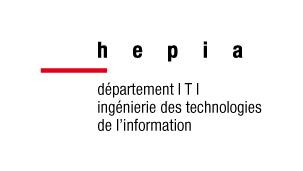
\includegraphics[width=5.86cm,height=3.31cm]{template/images/title/hepia_logo}};
\begin{spacing}{0.956}
\vspace{0.5cm}

%% CONTENT STARTS HERE
Durant ces dernières années, l'Intelligence Artificielle (IA) n'a fait que progresser et a révolutionné beaucoup de domaines comme le droit, le domaine médical, la biologie ou encore la musique. Ce travail est la continuité de mon travail précédent, dont le but était de détecter des notes de trompette sur une octave de Do. L'objectif du présent travail est d'utiliser différentes architectures de modèle connexionniste (réseau neuronal) et de voir s'il est possible de détecter des notes et accords de guitare pour des sons mono échantillonnés à 44.1[kHz]. De plus, il sera possible de considérer le signal dans le monde discret (échantillonné) et dans le monde fréquentiel. Ainsi, le but est de parvenir à une utilisation en temps réel avec le moins de latence possible (autant visuelle qu'auditive). Dans le monde de la musique, une latence supérieure à cinq millisecondes pour le traitement du signal (calculs) est indésirable et se fait fortement ressentir. Le challenge est donc que les architectures proposées prédisent le plus précisément possible l'accord ou la note jouée dans un temps inférieur à cinq millisecondes. Pour ce travail, j'ai dû également créer un ensemble de données en partant de zéro. Par rapport au temps et aux ressources mises à ma disposition, j'ai décidé de m'attaquer à la gamme tempérée de la musique occidentale (pas de musique microtonale) et de représenter les accords mineurs et majeurs à trois sons et les notes dans leurs différentes octaves pour l'accordage standard d'une guitare (Mi, La, Ré, Sol, Si, Mi). L'architecture m'ayant donné les meilleurs résultats, à savoir une précision moyenne de 95.51\%, utilise une transformée de Fourier rapide pour passer dans le monde des fréquences et est composée d'une cellule LSTM bidirectionnelle.

\vfill
\begin{center}
	{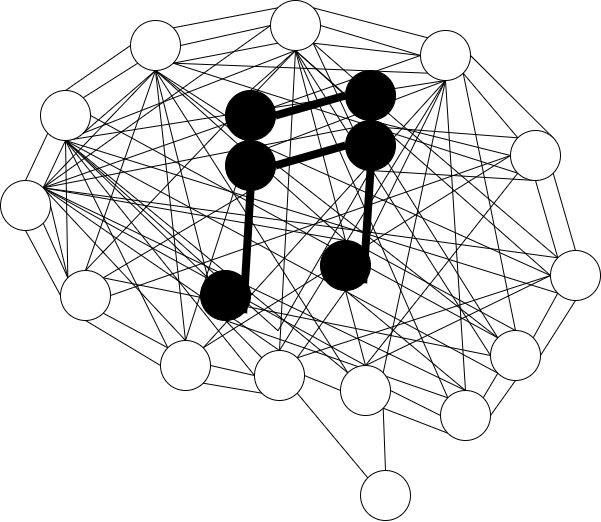
\includegraphics[height=5cm,width=5cm]{template/images/abstract/image}}\\*
\vfill
%% CONTENT ENDS HERE

\begin{center}
	{\sf
		%%%%%%%%%%%%%%%%%%%%%%%%%%%%%%%%%%%%%%%%%%%%%%%%%%%%%%%%%%%%%%%%%%%%%%%%%%%%%%%%
		%%%%%%%%%%%%%%%%%%%%%%%%%% DO NOT MODIFY THE TABLE BELOW %%%%%%%%%%%%%%%%%%%%%%%
		%%%%%%%%%%%%%%%%%%%%%%%%%%%%%%%%%%%%%%%%%%%%%%%%%%%%%%%%%%%%%%%%%%%%%%%%%%%%%%%%
		\begin{tabular*}{16cm}{p{7.7cm} p{7.7cm}}
			\small Candidat-e:					&	\small Professeur-e(s) responsable(s):\\*[10pt]
			\small\textbf{\textsc{\Author}}		&	\small\textbf{\textsc{\Professor}}\\*[10pt]
			\footnotesize  Filière d’études : ITI	&	\footnotesize  \textbf{En collaboration avec:} \textbf{\Client}\\*[10pt]
			\footnotesize  {} & \footnotesize  Travail de bachelor soumis à une convention de stage en entreprise: \textbf{\Convention}\\*[20pt]
			\footnotesize  {} & \footnotesize  Travail soumis à un contrat de confidentialité: \textbf{\Confidentiel}\\*[10pt]
		\end{tabular*}\\*[0.5cm]
	}
\end{center}

\end{center}
\end{spacing}
\end{document}
